\chapter{Lasso regression}
\label{ch:lasso}


The Lasso regression estimator, introduced in Tibshirani, 1996, is another estimator which, like the Ridge estimator, is particularly useful in situations when we have a large number of parameters and few observations. It works by identifying a sparse set of ``important'' predictors, and shrinks the coefficients of the remaining ``unimportant'' predictors to zero. While the Ridge estimator shrinks such coefficients towards zero (so that they are very small but not exactly zero), the Lasso estimator goes further and shrinks these coefficients so much that they become equal to zero. That is, while the Ridge estimator significantly reduces the influence of these ``unimportant'' predictors, the Lasso estimator removes them entirely. 

\section{The Lasso estimator}

Formally, given a regression problem $Y = X \beta + \epsilon$, the Lasso estimator is defined to be

\begin{equation}
\hat{\beta}_{lasso} = \underset{\beta}{\text{argmin }} \frac12 \|y - X \beta \|_2^2 \hspace{0.5cm} \text{subject to the constraint } ~~ \|\beta\|_1 = \sum_{j=1}^p |\beta_j| < \lambda
\end{equation}

where $\lambda$ is some tuning parameter that controls the amount of shrinkage that is applied to the estimates. \textcolor{red}{Write something about why we have the scaling factor of $\frac12$ - in another version I have a scaling factor of $\frac{1}{2n}$}. To put it a bit more simply, the Lasso estimator is essentially solving the standard OLS optimization problem while simultaneously ensuring that the sum of the absolute values of the coefficients does not get too large (this constraint is what forces many of the coefficients towards zero). In fact, this estimator is extremely similar to the Ridge estimator which can be reformulated as

\begin{equation}
\hat{\beta}_{ridge} = \underset{\beta}{\text{argmin }}  \|y - X \beta \|_2^2 \hspace{0.5cm} \text{subject to the constraint } ~~ \|\beta\|_2^2 = \sum_{j=1}^p \beta_j^2 < \lambda
\end{equation}


The key difference between Lasso and Ridge is that the Lasso estimate regularizes using the $L^1$ norm of $\beta$, while the Ridge regularizes using the $L^2$ norm of $\beta$. To understand why the Lasso will often produce coefficients that are exactly equal to zero (whereas ridge will not), we turn to Figure \ref{fig:ridge_lasso}. Note that the elliptical contours in Figure~\ref{fig:ridge_lasso} correspond to the the quadratic function $||y - X\beta||_2^2$, and we can see that they are centered at the OLS estimate, $\hat{\beta}$. This is a reflection that the OLS estimate is the equal to $\underset{\beta}{\text{argmin}}||y - X\beta||_2^2$. The constraint region for Lasso is presented by the solid black square in panel (a), while the constraint region for Ridge is the solid black circle in panel (b). The solution that arises from the Lasso estimator is given by the ``first'' position for which the elliptical contours touch the square; this position will sometimes occur at a corner, corresponding to a zero coefficient. For the Ridge estimator, however, there are no corners for the contours to hit and hence zero solutions will rarely result.




\begin{figure}[H]
\centering
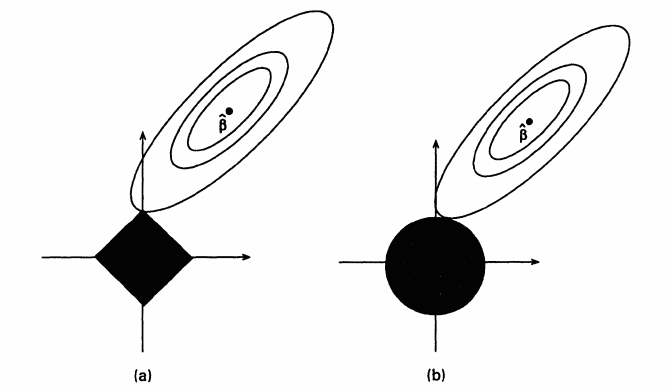
\includegraphics[scale=0.4]{lasso.png}
\caption{Estimation picture for (a) the lasso and (b) ridge regression. Figure from \emph{Regression shrinkage and selection via the lasso}, Tibshirani, 1996}
\label{fig:ridge_lasso}
\end{figure}


The formulation of the lasso can be re-written in a more familiar form as

\begin{equation}
\label{eq:lasso1}
\hat{\beta}_{lasso} = \underset{\beta}{\text{argmin}} \left[ \frac12 \| y - X \beta \|_2^2 + t \|\beta \|_1 \right]
\end{equation}

Let's consider the excruciatingly simple case where $p = n = 1$ (one observation and there are no predictor variables other than an intercept term). In this case, Equation~\ref{eq:lasso1} is simply 

$$\hat{\beta}_{lasso} = \underset{\beta}{\text{argmin}} \left[ \frac12 ( y -  \beta )^2 + t |\beta | \right].$$


Since we cannot differentiate $y = |x|$ at $x = 0$, we can instead consider the sub-derivative, $w$, of $y = |x|$ defined by

\begin{align*} 
w = 1 & ~\text{ if }~ x > 0 \\
w = -1 & ~\text{ if }~ x < 0\\
|w| \leq 1 & ~\text{ if }~ x = 0 
\end{align*}
so that we can determine the Lasso estimate by sub-differentiating $\frac12(y - \beta)^2 + \lambda | \beta|$ with respect to $\beta$. Setting the sub-derivative to zero yields

$$ 0 = - (y - \hat{\beta}_{lasso}) + \lambda w$$
where $w$ is the sub-derivative of $|\beta|$ described above. Solving this equation yields the solution

$$\hat{\beta}_{lasso} = \begin{cases} y - \lambda & \text{if } \hat{\beta}_{OLS} > 0\\
y + \lambda & \text{if } \hat{\beta}_{OLs} < 0\\
0 & \text{if } \hat{\beta}_{OLS} = 0
\end{cases}$$


in particular, we can write this more condensely as

$$\hat{\beta}_{lasso} = (|y| - \lambda) \times  sign(\hat{\beta}_{OLS}$$

\textcolor{red}{In my notes from last year this bit was very wrong... I've written here what I think it should be, but I've skipped a lot of the details that should be there...)}



Note that, similarly to the Ridge estimator, the Lasso estimate takes on a little bit of bias, but makes up for this in reducing the overall MSE by reducing the variance. Further, it is important to normalize the feature matrix, $X$ \textcolor{red}{why?}. Lasso and Ridge estimation can be implemented in R using the glmnet package.


\section{Estimation accuracy}

\textcolor{red}{In the November 13 and 18 classes from last year, there are a lot of technical details that I think might be a bit too much compared with the rest of the content of the book so far... so I haven't written it out here, but can do so if we decide it's important to do so...}